\documentclass[11pt,a4paper]{article}
\usepackage{float}
\usepackage[utf8]{inputenc}
\usepackage[left=2cm,right=2cm,text={18cm,24cm},top=2cm]{geometry}
\usepackage[czech]{babel}
\usepackage{graphicx}
\usepackage{verbatim}
\usepackage{svg}
\usepackage{rotating}
\usepackage{hyperref}
\usepackage{amsmath}
\usepackage[T1]{fontenc}
\usepackage{enumitem}

\renewcommand{\familydefault}{\sfdefault}

\begin{document}
\begin{titlepage}
    \begin{center}
        % FIT logo
        
\includegraphics[scale=0.65]{fit.pdf} \\
                
        \vspace{2cm}
        
        \Large{
Mikroprocesorové a vestavěné systémy \\
(IMP) 2024/2025
		}
						                
		\vspace{2cm}
\vspace{2cm}



		\vspace{2cm}
		      
		\huge{
			\textbf{
				ESP32: Měření srdečního tepu \\
				digitální senzor } \\}
				
							                
			\vspace{2cm}

			\Large{}
			\today{}
			
			\vspace{2cm}
			
			Marek Joukl \verb|xjoukl00|
			\end{center}
			\end{titlepage}
\pagebreak{}
    
\tableofcontents
    
\pagebreak{}

\section{Úvod}

Cílem projektu bylo vytvořit funkční měřič srdečního tepu za pomoci mikrokontroleru ESP32 na vývojové desce Wemos D1 R32, snímače srdečního tepu PulseSenzor a grafického OLED displeje SSD1306.

Projekt je implementován ve vývojovém prostředí Arduino IDE a jazyce C++ za použití knihoven Adafruit\_SSD1306.h, Adafruit\_GFX.h a Wire.h.

Program čte analogová data ze senzoru, filtruje signál a detekuje údery srdce, ze kterých vypočítá průměrný počet úderů za minutu (BPM) a vypíše na displej.

\section{Zapojení}

\underline{Pulse Senzor}
\begin{itemize}
    \item VCC $\rightarrow$ 5V (ESP32)
    \item GND $\rightarrow$ GND (ESP32)
    \item Signal $\rightarrow$ GPIO 36 (Analog input)
\end{itemize}

\underline{OLED Displej}
\begin{itemize}
    \item VCC $\rightarrow$ 5V (ESP32)
    \item GND $\rightarrow$ GND (ESP32)
    \item SCL $\rightarrow$ SCL (ESP32)
    \item SDA $\rightarrow$ SDA (ESP32)
\end{itemize}

 \begin{figure}[ht]
    \centering
    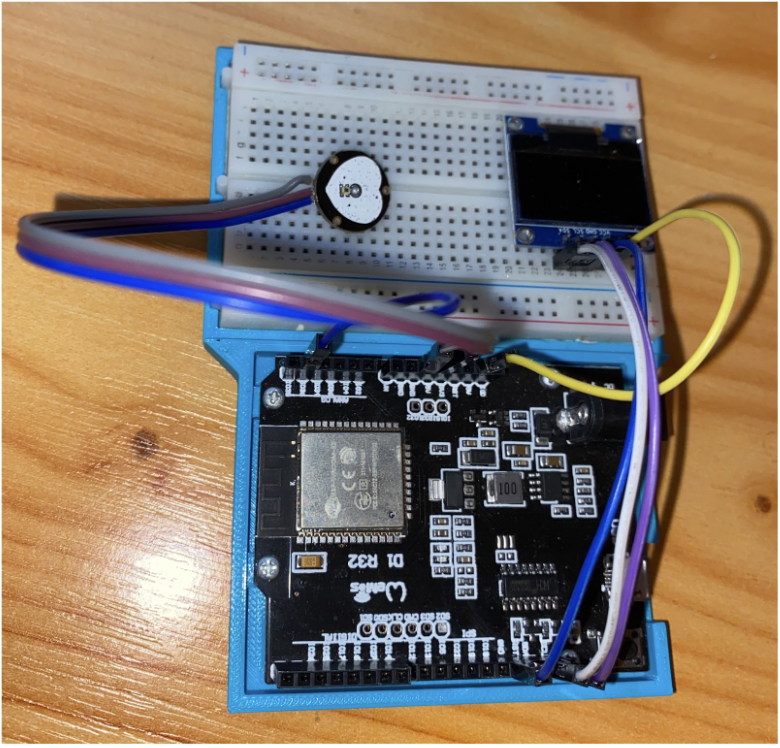
\includegraphics[width=0.6\linewidth]{zapojeni.png}
    \caption{Detail zapojení desky}
\end{figure}

\section{Implementace}

Snímač pulsu vysílá analogový signál, který kolísá v závislosti na srdečním tepu. ESP32 čte tento signál prostřednictvím svého ADC (analogově-digitálního převodníku). Pro vyhlazení signálu je použit dolnopropustný filtr (low-pass filter). Systém detekuje špičky (signály srdečního tepu) tak, že rozpozná, kdy signál překročí nastavený práh a následně opět klesne pod práh.

\subsection{Inicializace}
Ve funkci \texttt{setup()}, která se spouští při zapnutí zařízení, se nastaví BAUD rate, inicializuje OLED displej a zobrazí úvodní hláška. Dále je program ovládán z hlavní smyčky \texttt{loop()}. 

\subsection{Zpracování signálu}

V hlavní smyčce jsou data ze senzoru čtena pomocí funkce \texttt{analogRead()}, která jsou dále filtrována dolní propustí, což eliminuje náhodný šum a usnadňuje další zpracování signálu. Jednotlivé údery srdce jsou detekovány na základě překročení předem definované prahové hodnoty. Tato prahová hodnota je kalibrována na základě signálu v klidovém stavu, kdy senzor není v kontaktu s prstem (baseline), a hodnot signálu při úderech srdce.

Před samotným výpočtem BPM je ověřeno, že signál opět klesl pod prahovou hodnotu. Tímto způsobem se zajišťuje, že detekovaný úder srdce je skutečný a že nedošlo k falešné detekci způsobené šumem nebo náhodnými výkyvy v signálu.

Po potvrzení detekce platného úderu se spočítá časový interval mezi aktuálním úderem a posledním zachyceným úderem (tzv. beat interval). Tento interval je pak použit k výpočtu BPM pomocí vzorce
\[
BPM = \frac{60000}{\text{beatInterval}},
\]
kde \texttt{beatInterval} představuje časový rozdíl v milisekundách mezi dvěma po sobě jdoucími údery srdce. Pokud vypočtená hodnota BPM spadá do přijatelného rozmezí (40--200 BPM), je hodnota BPM považována za platnou a použije se jak pro okamžité zobrazení na OLED displeji, tak pro výpočet průměrného BPM (\texttt{avgBPM}). Průměrné BPM se počítá jako průběžný průměr všech detekovaných platných úderů:
\[
\texttt{avgBPM} = \frac{\texttt{totalBeats}}{\texttt{beatCount}}.
\]
Tímto způsobem je průměrné BPM neustále aktualizováno na základě všech zaznamenaných úderů srdce.

Pro zvýšení přesnosti je také zavedena proměnná \texttt{debounceTime}, která zabraňuje falešné detekci úderů během jedné periody srdečního cyklu.


\subsection{Vykreslování signálu}

Funkce \texttt{plotHeartbeat()} zajišťuje vykreslování průběhu srdečního tepu na OLED displeji pro příjemnější uživatelský zážitek. Každý nový bod grafu se vykreslí posunutím o 1 pixel doprava. Pokud graf dosáhne pravého okraje displeje, začne vykreslování znovu od levého okraje a starý grafický obsah se vymaže pomocí funkce \texttt{fillRect()}, čímž se udržuje čistý a aktuální vzhled.

Analogová hodnota signálu je převedena pomocí funkce \texttt{map()} do rozsahu, který odpovídá spodní polovině displeje (mezi \texttt{PLOT\_TOP} a \texttt{PLOT\_BOTTOM}). Tento proces zajišťuje, že grafický průběh nepřekrývá horní část displeje, kde jsou zobrazeny textové informace. Pokud je hodnota mimo tento rozsah, je automaticky omezena tak, aby se nevykreslovala mimo vymezenou oblast.

 \begin{figure}[ht]
    \centering
    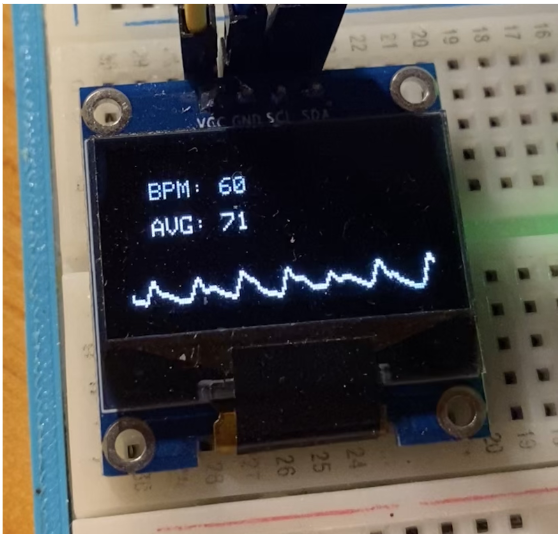
\includegraphics[width=0.4\linewidth]{display_plot.png}
    \caption{Detail zapojení desky}
\end{figure}

\pagebreak{}

\subsection{Spuštění}

Projekt je možné spustit v prostředí Arduino IDE. Je nutné mít nainstalované knihovny zmíněné v úvodu. Dále již stačí vybrat desku Wemos D1 R32 a správný port a nahrát program do zařízení tlačítkem Upload.

\section{Testování}

Správnost výstupu mého měřiče tepu byla ověřena srovnáním se senzorem zabudovaným v chytrých hodinkách. Testování probíhalo na dvou osobách, aby se zajistila spolehlivost zařízení u různých uživatelů a za různých fyzických podmínek. Hodnoty byly porovnávány jak v klidovém stavu, tak po fyzické námaze, kdy je tepová frekvence výrazně vyšší.

Toto opakované testování umožnilo důkladně zkontrolovat přesnost naměřených údajů a zajistit, že měřič poskytuje konzistentní výsledky. Výsledky z mého měřiče a hodinek byly zaznamenávány a porovnány, aby se zjistilo, zda naměřené hodnoty odpovídají. V následující tabulce jsou uvedeny příklady hodnot naměřených v různých podmínkách:

\begin{table}[H]
\centering
\begin{tabular}{|c|c|c|c|c|}
\hline
\textbf{Osoba} & \textbf{Klidový (můj)} & \textbf{Klidový (chytré hodinky)} & \textbf{Po cvičení (můj)} & \textbf{Po cvičení (chytré hodinky)} \\ \hline
1              & 62                     & 65                               & 112                       & 117                                   \\ \hline
2              & 71                     & 73                               & 132                       & 136                                   \\ \hline
\end{tabular}
\caption{Přehled naměřených hodnot ve vybraných situacích.}
\end{table}


\section{Videoukázka}

Demonstrace funkčnosti projektu dostupná zde: \\ \url{https://drive.google.com/file/d/1XfVxuwtyYrqaY6fT22sxy4qXZxiEHp-n/view?usp=sharing}.\\ Senzor a mikrokontroler je nejprve připojen k napájení, dále se zobrazí úvodní hláška a poté je zobrazena hlavní obrazovka s daty. Pro správné měření je nutné po přiložení prstu nejprve chvíli setrvat (10-15s), aby se senzor správně zkalibroval a zobrazoval validní údaje. Na konci videa je pro srovnání vidět hodnoty naměřené chytrými hodinkami.

\section{Závěr}
\subsection{Autoevaluace}

Celkové hodnocení je určeno dle rovnice hodnotícího klíče:
\[
\Sigma = (K1 + K2 \cdot F / 5) \cdot (E + F + Q + P + D),
\]
kde
\begin{itemize}
    \item \textbf{Konstanta K1} = 0.25
    \item \textbf{Konstanta K2} = 0.75

\item \textbf{Přístup k řešení E} = 2 \\
S řešením projektu jsem začal velmi brzy, což mi i přes problémy s nasazením a rozbitým senzorem (dráty vedoucí k senzoru se zlomily v části u senzoru, bylo nutné ve škole znovu zpájkovat) umožnilo projekt včas dokončit a odevzdat. Měl jsem zároveň dostatek času nejen splnit body dané v zadání, ale i zdokonalit vizuální stránku dodatečnou funkcí na vykreslování grafu, což senzor činí uživatelsky přívětivější.

    \item \textbf{Funkčnost řešení F} = 5\\
    Implementace splňuje všechny věci zmíněné v zadání. Měří tep, který zobrazuje na displeji zároveň s průměrným tepem.

    \item \textbf{Kvalita řešení Q} = 2\\
    Jak je popsáno i v části přístup, senzor je velice uživatelsky přívětivý a je jednoduché ho spustit. Stačí nahrát implementaci dle bodu 3.4. Zdrojový kód je přehledný a patřičně okomentovaný dle zásad správného programování.

    \item \textbf{Prezentace P} = 2\\
    Videoukázka je důkazem, že vše funguje jak má.

    \item \textbf{Dokumentace D} = 3\\
    Dokumentace obsahuje veškeré informace potřebné k pochopení, zapojení i vyzkoušení projektu. Je také typograficky kvalitně zpracovaná.
\end{itemize}

\[
\Sigma = (0.25 + 0.75 \cdot 5 / 5) \cdot (2 + 5 + 2 + 2 + 3) = \textbf{14}
\]

\section{Zdroje}

\begin{enumerate}[]
    \item \href{https://lastminuteengineers.com/pulse-sensor-arduino-tutorial/}{https://lastminuteengineers.com/pulse-sensor-arduino-tutorial/}
    \item \href{https://github.com/adafruit/Adafruit-GFX-Library}{https://github.com/adafruit/Adafruit-GFX-Library}
    \item \href{https://github.com/adafruit/Adafruit_SSD1306}{https://github.com/adafruit/Adafruit\_SSD1306}
\end{enumerate}


\end{document}
